\subsection{Reservoir computing}
A big disconnect between machine learning and how we perceive human reasoning is
how to solve and encode problems of temporal nature.
While feed forward structures which can only consider their current input can be
extended to reduce temporal problems into structural ones by adding delays
\cite{schrauwen_overview_2007}, a more natural approach is to use
recurrent structures that modify themselves in response to input.
A widely studied example of this approach is the recurrent neural network,
however the increase in expressiveness makes these structures very hard to train\cite{bertschinger_real-time_2004}.
Another example are random boolean networks \cite{gershenson_introduction_2004} studied by Kauffman as a
model for genetic regulatory networks.
Common for these two systems, and many more such as cellular
automata \cite{sipper_emergence_1999} and liquid state machines exhibit the
properties of \textit{complex systems} \cite{langton_computation_1990}.
Complex systems are systems that are, in a sense, magic.
In order to harness the power of these complex systems it is fruitless to
attempt to shape the topology and dynamics of the systems towards some specific
goal. Instead, the complex systems are used as \textit{reservoirs} which we will
interact with using a simple linearly separable input and output processing
layer which can be easily trained. \cite{schrauwen_overview_2007}
TO-DO: back linearly separable claims.
\subsection{Neurons}
Neurons are vastly complex entities, communicating through complex electric
and chemical signals. However, since we are more interested in the emergent
properties of neurons in the context of reservoir computing a superficial
description suffices.
We will only consider a generalized version of the neuron, but in our
experiments a plethora of different neurons are used, although they
all share the basic similarities described here.
The anatomy of a neuron is shown in \ref{fig:neuron_anatomy} and can roughly be
divided into the following parts:
\subsubsection{Soma}
The main body of the neuron. While we will view neurons as simple network nodes
it is important to note that the neuron is highly complex, it can blah blah
\subsubsection{Dendrites}
To sense its surroundings the neuron is equipped with dendrites. These
branching structures act as receivers, propagating electro-chemical stimuli to
the cell body. Their reach is only to the immediate vicinity of the cell, they
do not form longer connections.
\subsubsection{Axon}
The axon is a long tendril, extending over a meter in the case of the sciatic
nerve TO-DO maybe embed link? which transmits information as electrical pulses
to other neurons. An axon can branch off and reach multiple neurons, it is not a
one to one connection.
\subsection{The NTNU Cyborg Project}
\subsection{MEA2100}
To perform experiments a MEA2100 system has been purchased from multichannel systems.
The MEA2100 system is built to conduct experiments on in-vitro cell cultures, 
with the main focus being on neurons.
The principal components of the MEA2100 systems are:
\subsubsection{Micro electrode array}
\begin{figure}[h!]
    %\centering
    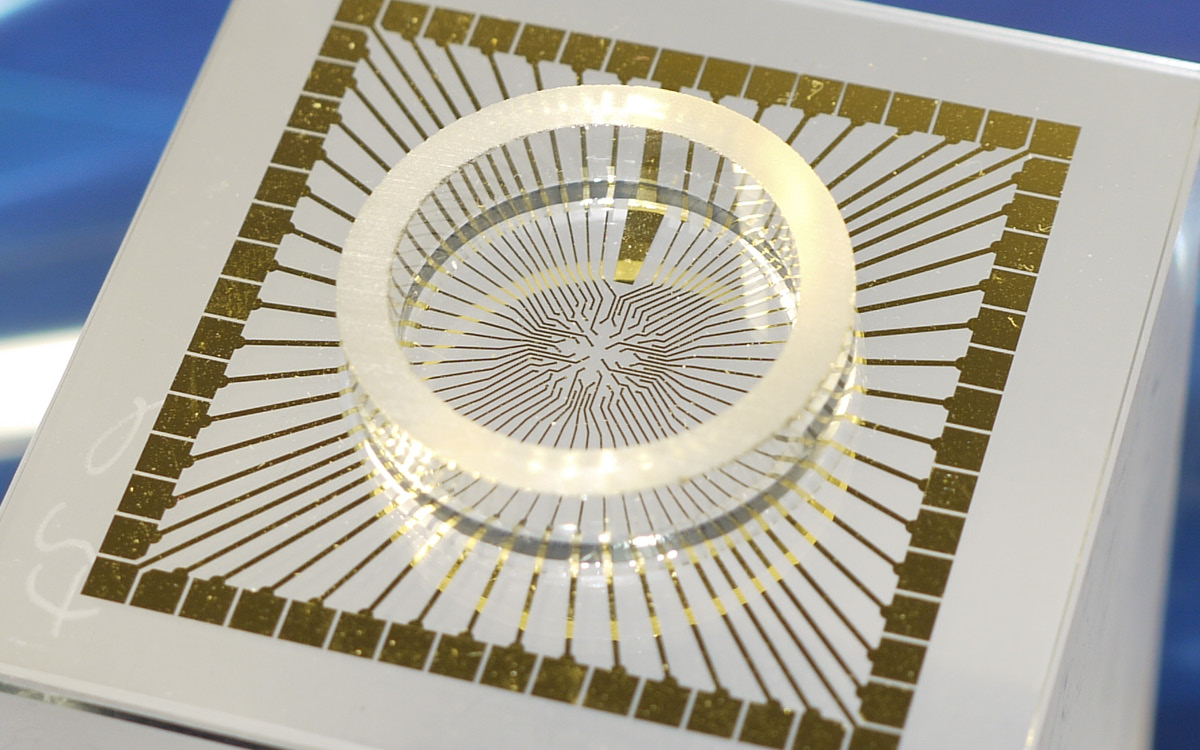
\includegraphics[width=\linewidth]{images/MEA.jpg}
    \caption{A generic MEA}
    \label{fig:generic_MEA}
\end{figure}
To experiment on the properties of cells or other electrically active subjects the
micro electrode array (MEA) is used. As the name implies the MEA is equipped with
an array of electrodes able to both measure the electrical properties of the 
experiment subjects, as well as applying outside stimuli, acting in a sense as
output and input for the subject. \ref{fig:generic_MEA} shows an empty MEA,
\ref{st_olav_MEA} shows an MEA from st.olavs with a live neuron culture.
\begin{figure}[h!]
    %\centering
    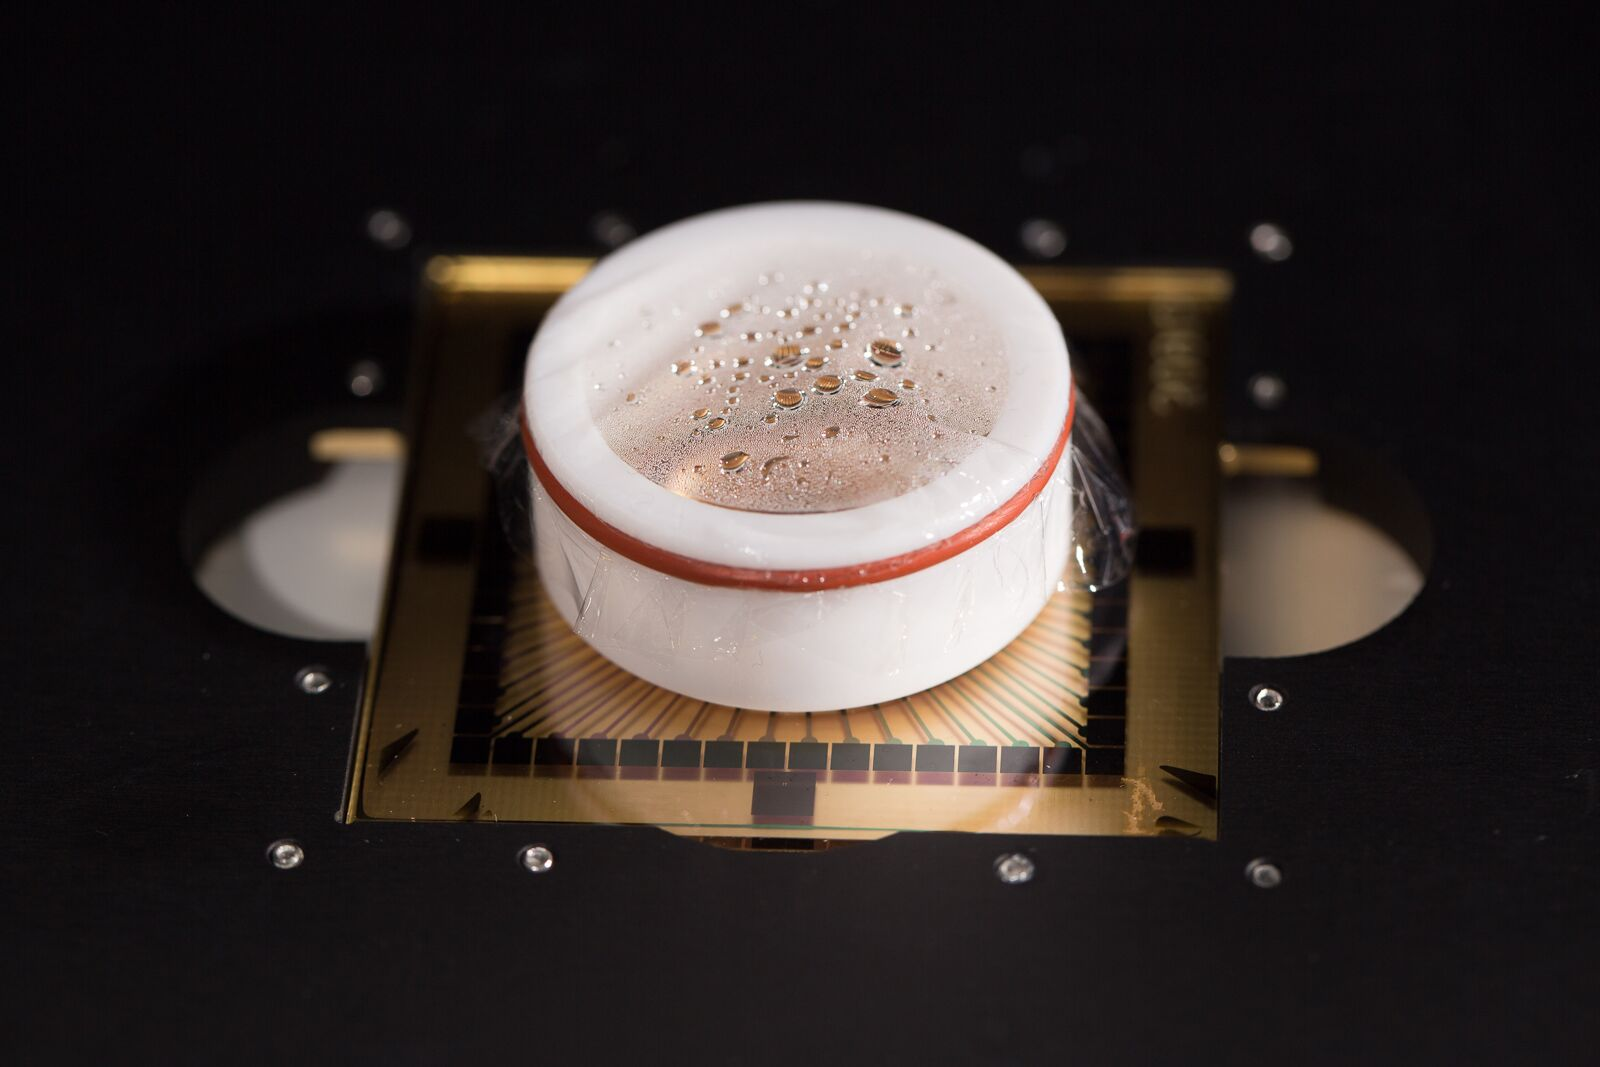
\includegraphics[width=\linewidth]{images/st-olavs-mea.jpg}
    \caption{A MEA with a live culture, photographed by Kai}
    \label{fig:st_olav_MEA}
\end{figure}
\subsubsection{Headstage}
The electrodes of the MEAs are measured and stimulated by the headstage which
contains the necessary high precision electronics needed for microvolt range readings.
\ref{fig:headstage} shows the same type of headstage used in this paper along
with an MEA.
\begin{figure}[h!]
    %\centering
    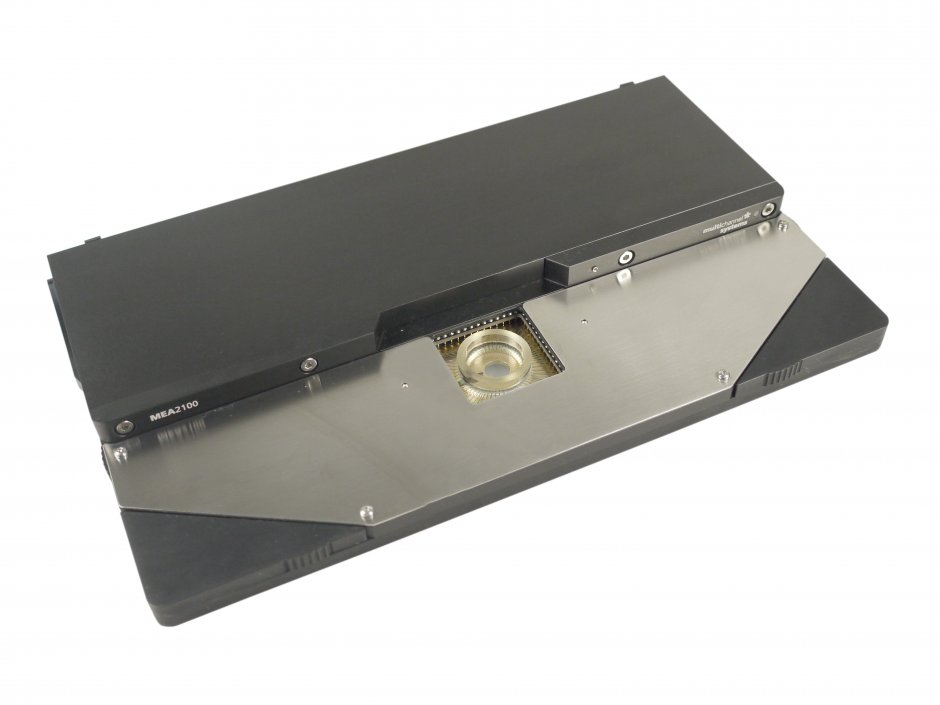
\includegraphics[width=\linewidth]{images/MEA2100-HS60.jpg}
    \caption{The headstage}
    \label{fig:headstage}
\end{figure}
\subsubsection{Interface board}
The interface board connects to up to two head-stages and is responsible for interfacing
with the data acquisition computer, as well as auxiliary equipment such as temperature
controls.
\begin{figure}[h!]
    %\centering
    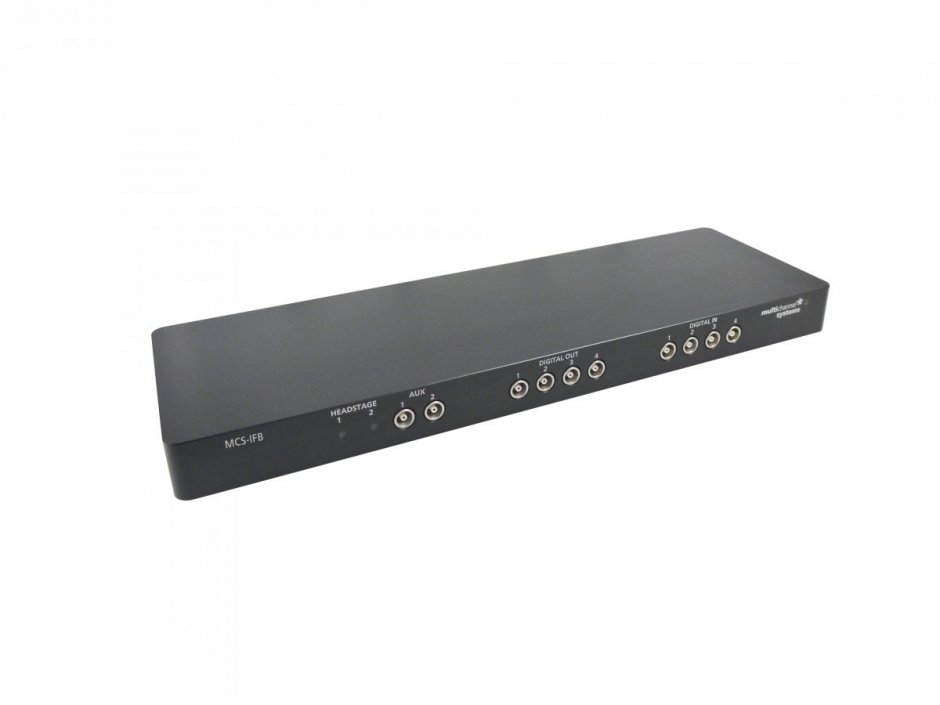
\includegraphics[width=\linewidth]{images/MCS-IFB.jpg}
    \caption{The MCS interface board}
    \label{fig:neuron_anatomy}
\end{figure}
The interface board has two modes of operation.
In the first mode the interface board processes and filters data from up to two
headstages as shown in \ref{fig:IFB_regular} which can then be acquired on a normal
computer connected via USB.
In the second mode of operation a Texas instruments TMS320C6454 digital signal
processor is activated which can then be interfaced with using the secondary USB
port as shown in \ref{fig:IFB_BSP}
\begin{figure}[h!]
    %\centering
    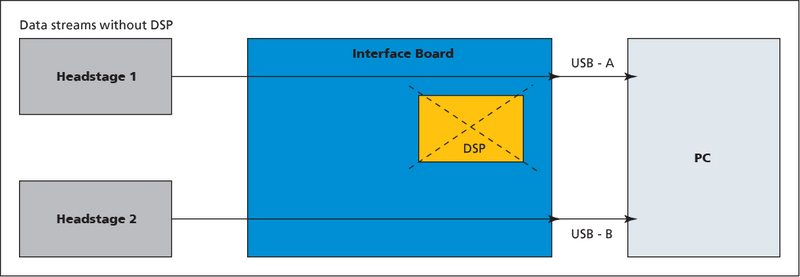
\includegraphics[width=\linewidth]{images/regular_operation.png}
    \caption{Casual mode}
    \label{fig:IFB_regular}
\end{figure}
%% %% %% %% %% %% %% %% %% %% %% %% %% %% %% %% %% %% %% %% %% %% %% %% %% %%
%% %% %% %% %% %% %% %% %% %% %% %% %% %% %% %% %% %% %% %% %% %% %% %% %% %%
%% %% %% %% %% %% %% %% %% %% %% %% %% %% %% %% %% %% %% %% %% %% %% %% %% %%
%% %% %% %% %% %% %% %% %% %% %% %% %% %% %% %% %% %% %% %% %% %% %% %% %% %%
\begin{figure}[h!]
    %\centering
    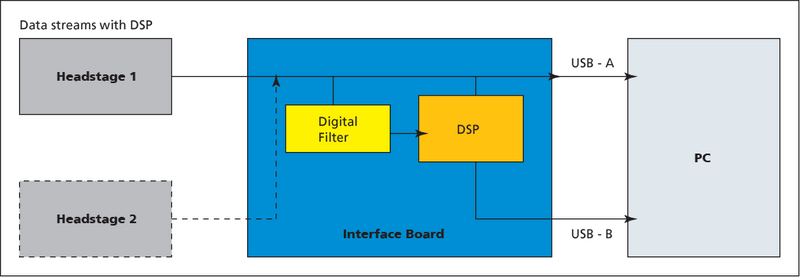
\includegraphics[width=\linewidth]{images/dsp_operation.png}
    \caption{DSP active}
    \label{fig:IFB_DSP}
\end{figure}
%% %% %% %% %% %% %% %% %% %% %% %% %% %% %% %% %% %% %% %% %% %% %% %% %% %%
%% %% %% %% %% %% %% %% %% %% %% %% %% %% %% %% %% %% %% %% %% %% %% %% %% %%
%% %% %% %% %% %% %% %% %% %% %% %% %% %% %% %% %% %% %% %% %% %% %% %% %% %%
%% %% %% %% %% %% %% %% %% %% %% %% %% %% %% %% %% %% %% %% %% %% %% %% %% %%
\begin{figure*}[p]
    \centering
    \includegraphics[width=\textwidth]{images/"Neuron anatomy".png}
    \caption{a neuron}
    \label{fig:neuron_anatomy}
\end{figure*}
%%% Local Variables:
%%% mode: latex
%%% TeX-master: "../main"
%%% End:
